\chapter{Programas utilizados}

\section{Entorno de programación - Visual Studio Code}

Existen muchos entornos de programación disponibles, el utilizado para el proyecto fue Visual Studio Code \cite{visual_studio_code}. El mismo fue utilizado porque es gratuito y se encuentra disponible para Windows, Linux y Mac.

Visual Studio Code es un entorno de desarrollo flexible que cuenta con extensiones que pueden ser instaladas para ayudar con la escritura y visualización de código. En la figura~\ref{F:vsc_extensions} se encuentran capturas de pantalla del entorno de programación, indicando con flechas numeradas la secuencia para encontrar las dos extensiones utilizadas.

\begin{figure}[ht!]
\centering
\subfloat[Extensión para visualización en Assembler]{
	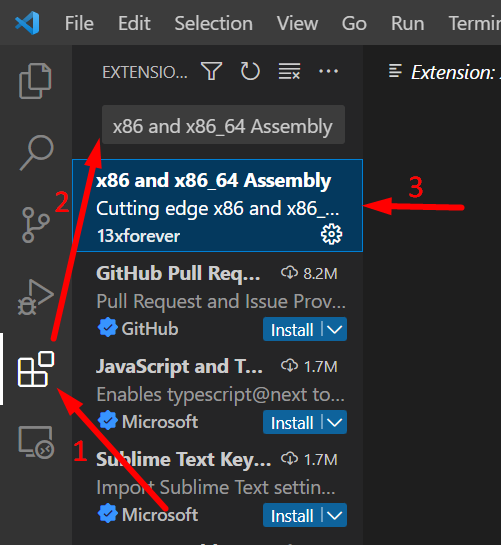
\includegraphics[width=0.4275\textwidth]{./imagenes/vsc_assembly_ext.png}
	\label{F:vsc_assembly_ext}}
\quad
\subfloat[Extensión para visualización de formato Intel]{
	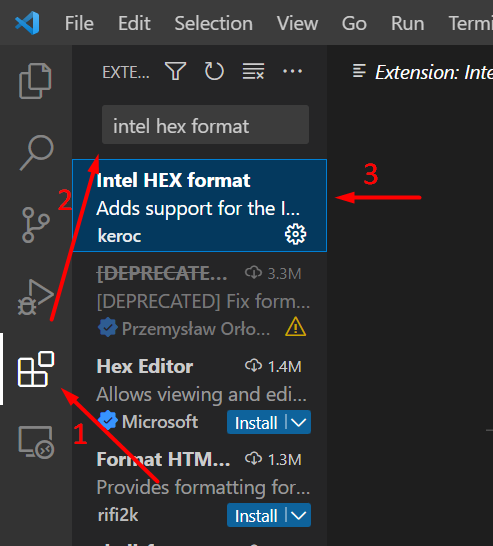
\includegraphics[width=0.42275\textwidth]{./imagenes/vsc_intel_ext.png}
	\label{F:vsc_intel_ext}}
\caption{Extensiones utilizadas en Visual Studio Code}
\label{F:vsc_extensions}
\end{figure}

La primera de ellas, \entreComillas{x86 and x86\_64 Assembly}, es una extensión para el resaltado de sintaxis. En la figura~\ref{F:snyntax_highlighting} puede apreciarse un programa sencillo que hace parpadear el LED Q en un sistema con el CDP1802, donde lo más importante es la diferencia de color entre las instrucciones y los comentarios, lo cual facilita la lectura y análisis del código.

\begin{figure}[ht!]
  \centering
  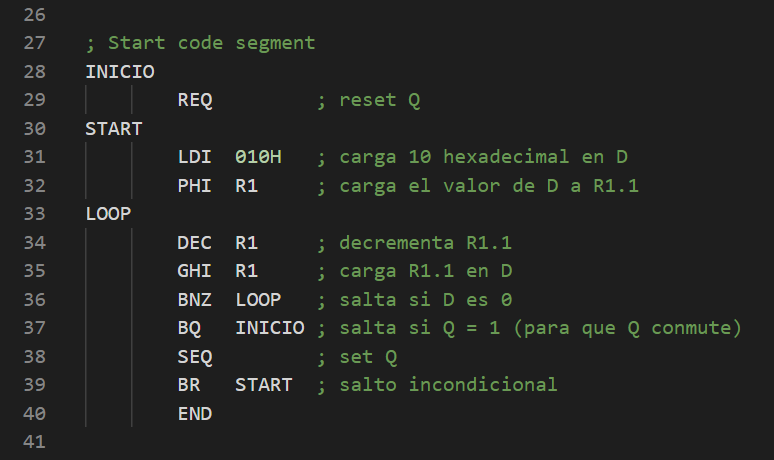
\includegraphics[width=.75\textwidth]{./imagenes/syntax highlishtpng.png}
  \caption{Extensión para resaltar sintaxis de código en assembler}
  \label{F:snyntax_highlighting}
\end{figure}

La segunda extensión es \entreComillas{Intel HEX format}, dedicada a resaltar la composición de archivos en formato Intel, lo cual sería difícil de otro modo, o requeriría un programa específico para esta tarea. En la figura~\ref{F:intel_highlighting} se encuentra una captura de pantalla de un archivo Intel visualizado con esta extensión. En el anexo~\ref{C:anexo_formato_intel} (\nameref{C:anexo_formato_intel}) se encuentra descrito el formato Intel.

\begin{figure}[ht!]
  \centering
  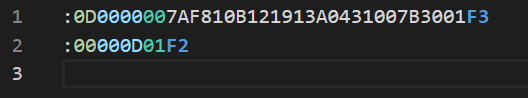
\includegraphics[width=0.57\textwidth]{./imagenes/intel_format_highlighting.png}
  \caption{Extensión para resaltar la composición de archivos en formato Intel}
  \label{F:intel_highlighting}
\end{figure}

\section{Revisión de modificaciones con Git y Visual Studio Code}

Cuando se tienen programas grandes y se sabe que se han realizado modificaciones, intentar encontrarlas y ver nada más estos cambios puede resultar una tarea engorrosa. Sin embargo, existen herramientas para poder visualizar cambios realizados en un código. Una de estas herramientas es Git, un programa para llevar el control de versión del desarrollo de código. Git es un programa con muchas funciones, pero la única que es de interés en este momento es la revisión de diferencias entre dos archivos.

Para utilizar esta herramienta primero debe descargarse Git desde \cite{git_download}, y una vez instalado se requiere una pequeña configuración, la cual puede verse en el video tutorial \cite{git_difftool_config}, pero de igual manera se describe a continuación.

Primero debe abrirse Git, para ello debe hacerse click derecho en una parte vacía de un directorio cualquiera, también puede ser el escritorio, y hacer click en \entreComillas{Git Bash Here}, como puede verse en la figura~\ref{F:git_inst_1}. Luego, en la ventana del programa, escribir los comandos como se muestran en la figura~\ref{F:git_inst_2}.

\begin{figure}[ht!]
\centering
\subfloat[Abrir Git]{
	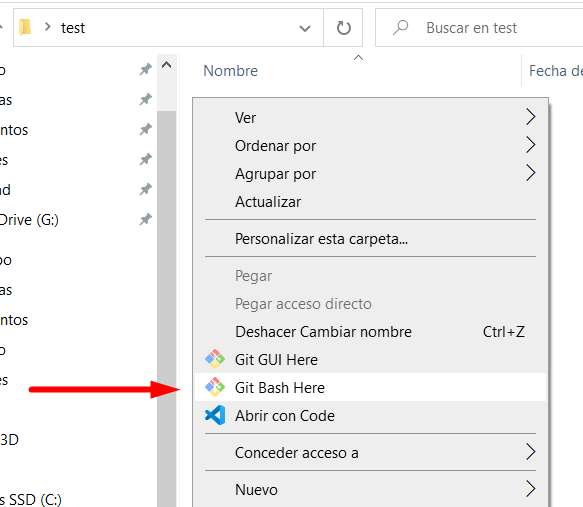
\includegraphics[width=0.57\textwidth]{./imagenes/git_inst_1.png}
	\label{F:git_inst_1}}
\\
\subfloat[Comandos para la configuración inicial]{
	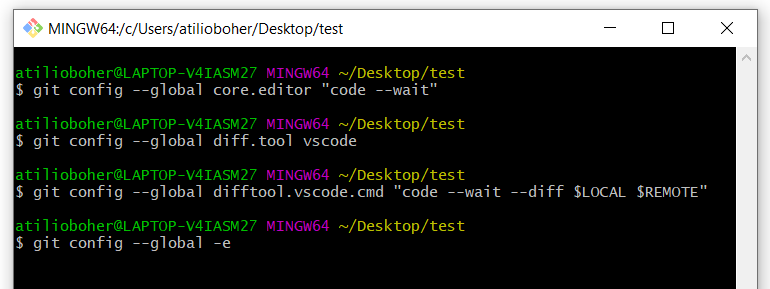
\includegraphics[width=0.8\textwidth]{./imagenes/git_inst_2.png}
	\label{F:git_inst_2}}
\caption{Configuración inicial de Git}
\label{F:git_inst}
\end{figure}

Al ejecutar el último comando, Visual Studio Code se abrirá, y la configuración realizada debería verse como en la figura~\ref{F:git_inst_3}, de no ser así, debe rellenarse lo faltante, guardar el archivo y cerrar el programa.

\begin{figure}[ht!]
  \centering
  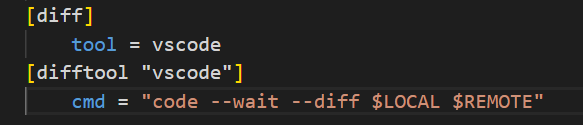
\includegraphics[width=0.57\textwidth]{./imagenes/git_inst_3.png}
  \caption{Configuración de Git relacionada a difftool}
  \label{F:git_inst_3}
\end{figure}

Una vez hecho todo esto, Git se encuentra configurado y se pueden comparar dos archivos simplemente abriendo Git, como ya se indicó en la figura~\ref{F:git_inst_1}, y escribiendo el comando que se observa en la captura de la figura~\ref{F:git_inst_4}, donde los dos últimos parámetros son los nombres de los archivos a comparar (en este caso \texttt{test.asm} y \texttt{test\_modificado.asm}).

\begin{figure}[ht!]
  \centering
  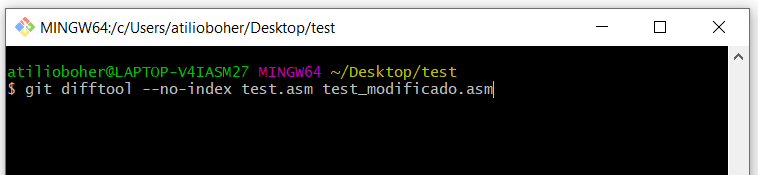
\includegraphics[width=0.8\textwidth]{./imagenes/git_inst_4.png}
  \caption{Comando para comparar dos archivos con Git}
  \label{F:git_inst_4}
\end{figure}

En la figura~\ref{F:git_difftool_exemple} puede apreciarse la diferencia entre los códigos, en este caso es una simple diferencia ilustrativa.

\begin{figure}[ht!]
  \centering
  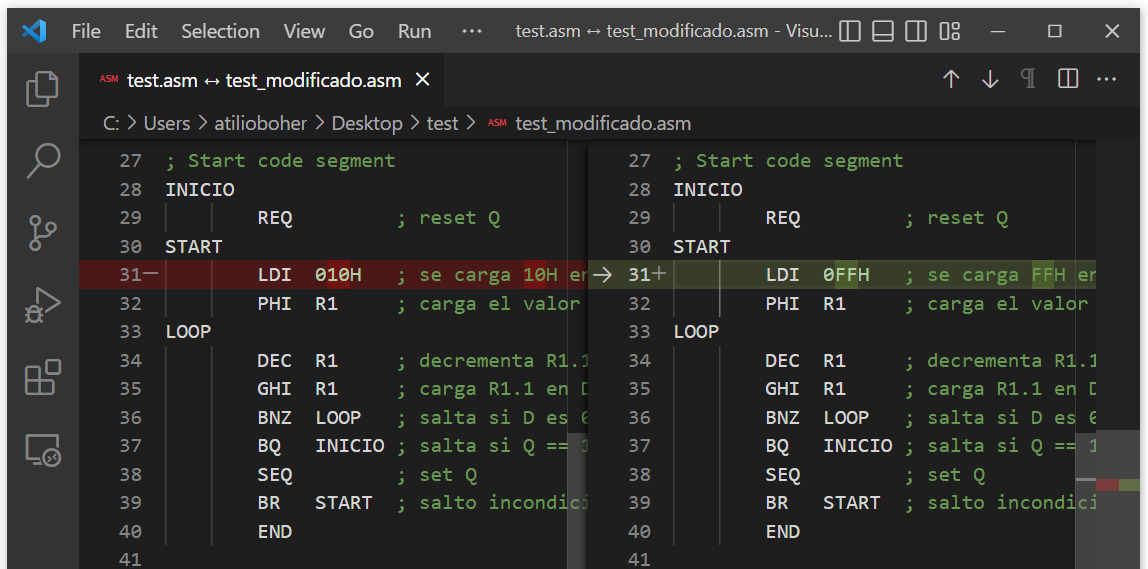
\includegraphics[width=0.99\textwidth]{./imagenes/git_difftool_exemple.png}
  \caption{Ejemplo de comparación}
  \label{F:git_difftool_exemple}
\end{figure}

Lo útil de esta herramienta es que no solo indica la línea, sino también el lugar exacto del cambio o diferencia.

\section{Ensamblador A18}
\label{C:a18}

El ensamblador utilizado se denomina A18 y fue encontrado en \cite{a18} donde se encuentra el enlace para poder descargarlo. Con el mismo es posible ensamblar código assembler del CDP1802 (con los mnemónicos indicados en su hoja de datos \cite{cdp1802_datasheet}) y obtener los archivos en formato Intel (\texttt{.hex}) y el listing (\texttt{.lst}). Además cuenta con un manual donde se indica cómo utilizarlo y todos los tipos de errores que pueden encontrarse a la hora de realizar el ensamblado.

Para utilizarlo es necesario tener el archivo \texttt{a18.exe} en el mismo directorio que el código \texttt{.asm} que busca ensamblarse. Luego, manteniendo apretado Shift izquierdo, se debe hacer click en una parte vacía del directorio y luego seleccionar \entreComillas{Abrir la ventana de PowerShell aquí}, como se aprecia en la figura~\ref{F:a18_1} (es posible que en vez de PowerShell diga Command Prompt, cualquiera sea el caso, se prosigue de la misma manera), esto abre una ventana de comandos en el directorio en cuestión.

\begin{figure}[ht!]
  \centering
  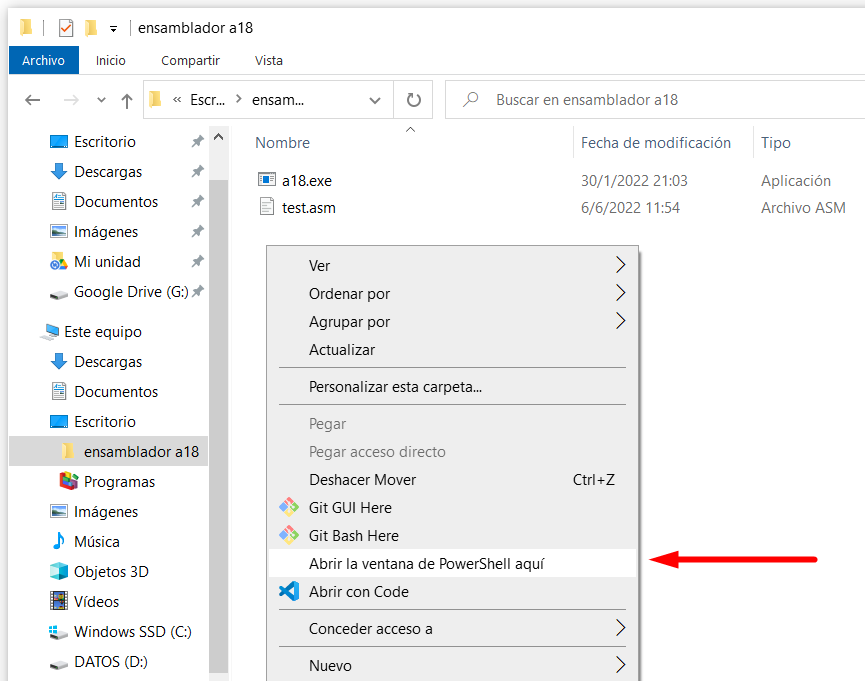
\includegraphics[width=0.75\textwidth]{./imagenes/a18_1.png}
  \caption{Apertura de ventana de comandos en directorio}
  \label{F:a18_1}
\end{figure}

En la ventana de comandos se deben reemplazar los nombres correspondientes; el primero es el nombre del programa a ensamblar, en formato \texttt{.asm}, el segundo es el nombre del archivo \texttt{.hex} a generar, y el último es el nombre del archivo listing, en formato \texttt{.lst}.

\vspace{0.75cm}
\footnotesize
\texttt{./a18.exe <nombre-de-archivo>.asm -o <nombre-de-archivo>.hex -l <nombre-de-archivo>.lst}
\normalsize
\vspace{0.75cm}

En la figura~\ref{F:a18_2} puede verse el resultado del ensamblado de un programa y si el mismo posee errores, es indicado al ejecutar el comando. En el archivo listing generado se encuentran indicadas las líneas que poseen errores, utilizando un código para identificar cada tipo de error, de manera que los detalles sobre los mismos pueden ser encontrados en el manual del ensamblador, que como ya se mencionó, puede encontrarse en la página \cite{a18}.

\begin{figure}[ht!]
  \centering
  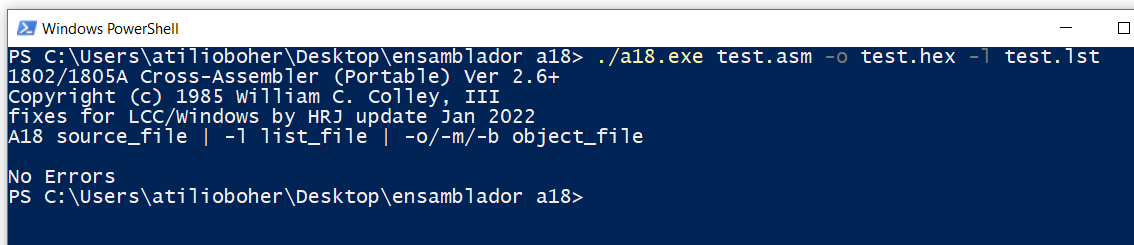
\includegraphics[width=0.95\textwidth]{./imagenes/a18_2.png}
  \caption{Resultado del ensamblado en ventana de comandos}
  \label{F:a18_2}
\end{figure}

Escribir este comando puede resultar engorroso. Por lo cual se escribió un pequeño script Batch, cuyas instrucciones se encuentran en la figura~\ref{F:a18_3}. Este script Batch se puede ejecutar con doble click y ensambla el código. Para ello el archivo Batch \texttt{.bat} debe tener el mismo nombre que el archivo \texttt{.asm} a ensamblar. En la figura~\ref{F:a18_4} se encuentra una captura de pantalla de los archivos necesarios, al hacer doble click en \texttt{test.bat}, se abrirá una ventana de comandos y \texttt{test.asm} se ensamblará automáticamente, sin necesidad de escribir ningún comando.

\begin{figure}[ht!]
\centering
\subfloat[Instrucciones Batch para el ensamblado con doble click]{
	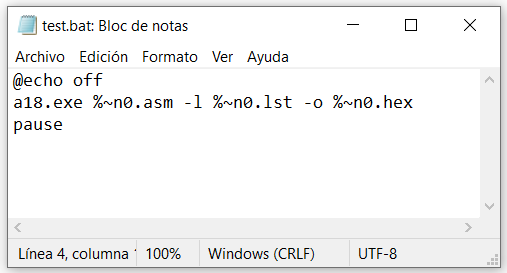
\includegraphics[width=0.47\textwidth]{./imagenes/a18_3.png}
	\label{F:a18_3}}
\quad
\subfloat[Uso del archivo \texttt{.bat}]{
	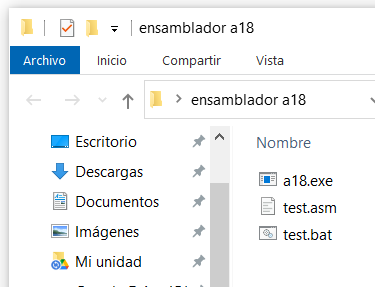
\includegraphics[width=0.39\textwidth]{./imagenes/a18_4.png}
	\label{F:a18_4}}
\caption{Ensamblado con script Batch}
\label{F:a18_5}
\end{figure}

\clearpage
\section{Emulador Emma02}

Existe un software llamado Emma02, el cual puede encontrarse en su página oficial \cite{emma_02}. El mismo permite la simulación de varios modelos de computadoras basadas en el microprocesador CDP1802. En la figura~\ref{F:emma02_interfas} puede apreciarse la variedad de computadoras disponibles, sin embargo, la más utilizada fue el Membership Card, seguida del Netronics Elf II.

\begin{figure}[ht!]
  \centering
  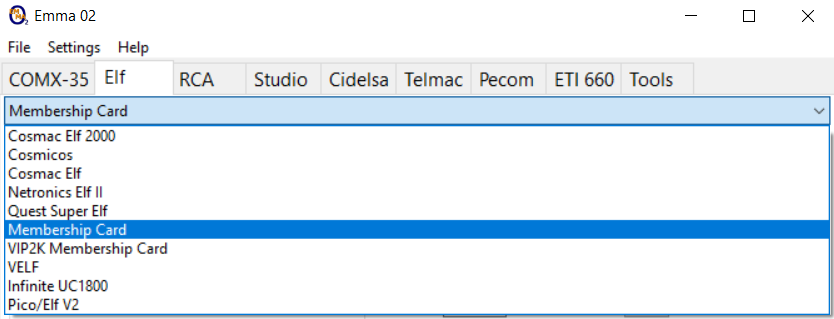
\includegraphics[width=0.85\textwidth]{./imagenes/emma02_interfaz.png}
  \caption{Computadoras disponibles que utilizan el CDP1802}
  \label{F:emma02_interfas}
\end{figure}

El simulador cuenta con programas ya disponibles para cada computadora. Para utilizar uno, debemos seleccionarlo en la solapa que se indica en la figura~\ref{F:emma02_1}; pero hay que tener en cuenta que quizás requiera cambiar alguna configuración de la computadora, como seleccionar la velocidad de transmisión correcta, el mapa de memoria, la dirección donde el microprocesador comenzará a ejecutar el programa, etc.

\begin{figure}[ht!]
  \centering
  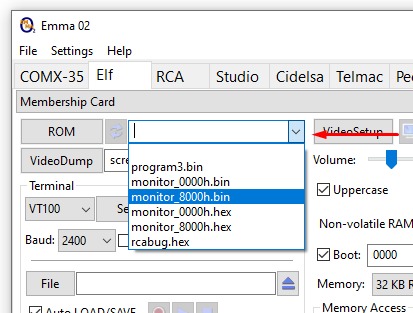
\includegraphics[width=0.5\textwidth]{./imagenes/emma02_1.png}
  \caption{Seleccionar programa}
  \label{F:emma02_1}
\end{figure}

Además, existe una forma de seleccionar programas ya disponibles en el simulador junto a la configuración específica necesaria para su funcionamiento, para ello hay que ir a File->Configuration->Load, como se indica en la figura~\ref{F:emma02_2}, para el caso de la computadora Netronics~Elf~II.

\begin{figure}[ht!]
  \centering
  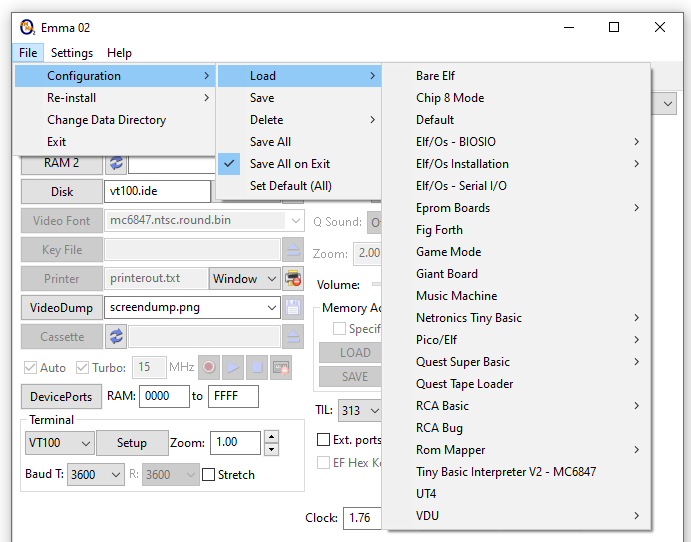
\includegraphics[width=0.89\textwidth]{./imagenes/emma02_2.png}
  \caption{Seleccionar programa y configuración}
  \label{F:emma02_2}
\end{figure}

Algunos de estos programas se encuentran en formato \texttt{.bin} y otros en formato \texttt{.hex}. Además, algunos también poseen el código fuente \texttt{.asm} en la carpeta contenedora. Para acceder a esta carpeta podemos hacer click en \entreComillas{ROM}, como se indica en la figura~\ref{F:emma02_ROM}. Esto abrirá una ventana para seleccionar un archivo \texttt{.hex} o \texttt{.bin}, y en esta ventana puede verse el directorio del emulador donde se encuentran los programas disponibles.

En este directorio (hay uno por cada modelo de computadora) pueden agregarse programas obtenidos en línea, o escritos y ensamblados por uno mismo para ser probados.

\begin{figure}[ht!]
  \centering
  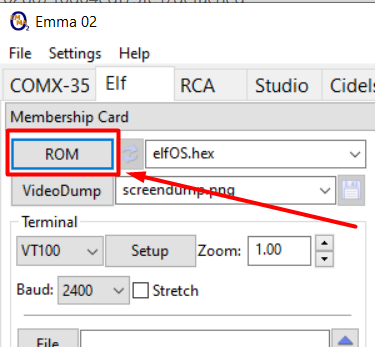
\includegraphics[width=0.37\textwidth]{./imagenes/emma02_cargar_hex.png}
  \caption{Seleccionar programa en Emma02}
  \label{F:emma02_ROM}
\end{figure}

El emulador también provee una herramienta denominada \entreComillas{Direct Assembler} (ver figura~\ref{F:emma02_direct_asm}), la cual muestra el código del programa en lenguaje assembler; puede ensamblar y desensamblar. Sin embargo, en este proyecto, se utilizó únicamente como herramienta de depuración de código y para el ensamblado se utilizó el ensamblador A18, ya expuesto en la sección~\ref{C:a18}.

\begin{figure}[ht!]
  \centering
  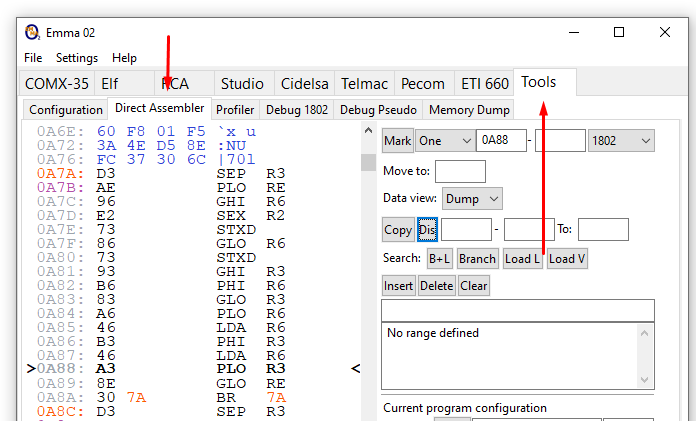
\includegraphics[width=0.8\textwidth]{./imagenes/emma02_direct_asm.png}
  \caption{Direct Assembler}
  \label{F:emma02_direct_asm}
\end{figure}

También existe una pestaña donde puede visualizarse los registros internos del microprocesador, y haciendo click en el botón \entreComillas{Trace} (figura~\ref{F:emma02_trace}), se registran todas las instrucciones ejecutadas, pudiendo luego copiar y pegar esto en un documento de texto para analizar detenidamente la ejecución de una secuencia de código.

\begin{figure}[ht!]
  \centering
  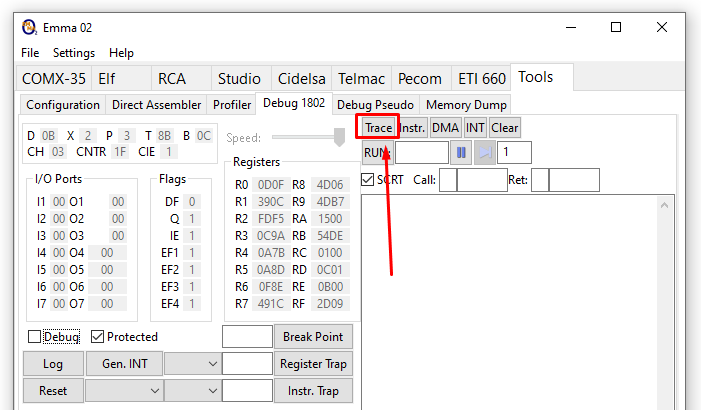
\includegraphics[width=0.8\textwidth]{./imagenes/emma02_trace.png}
  \caption{Registrar instrucciones ejecutadas y visualización de Registros internos}
  \label{F:emma02_trace}
\end{figure}

En la figura~\ref{F:emma02_trace_1} se encuentra una captura de instrucciones registradas con la herramienta \entreComillas{Trace}, en rojo se marcó una instrucción de escritura en memoria como ejemplo para ver cómo puede visualizarse información de interés, en este caso, tanto la dirección de memoria que fue escrita como el dato escrito en ella.

\begin{figure}[ht!]
  \centering
  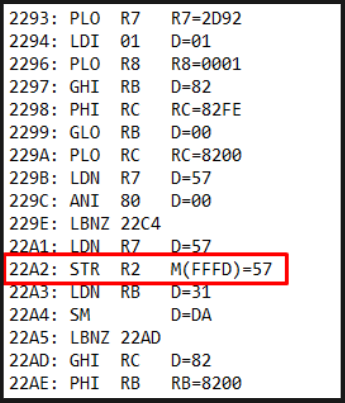
\includegraphics[width=0.38\textwidth]{./imagenes/emma02_trace_1.png}
  \caption{Captura de instrucciones ejecutadas}
  \label{F:emma02_trace_1}
\end{figure}

Estas características y herramientas mencionadas fueron las más utilizadas, sin embargo, se encuentran descritos más detalles de estas herramientas y otras más en la sección de ayuda de la página del emulador \cite{emma_02_help}.

\clearpage
\section{Terminal Tera Term}

Para la comunicación con la computadora se utiliza una terminal externa, en este caso se utilizó el programa Tera Term\copyright\cite{teraterm} ejecutándose en un ordenador personal. El mismo es sencillo de usar, sin embargo, se mencionan algunas configuraciones que se hicieron para volver más fácil su uso.

En la figura~\ref{F:teraterm_font} se puede ver la configuración realizada para tener un tamaño de letra más grande, debido a que la configuración por defecto es muy chica. Esta ventana de configuración puede encontrarse en Setup->Font->Font...

\begin{figure}[ht!]
  \centering
  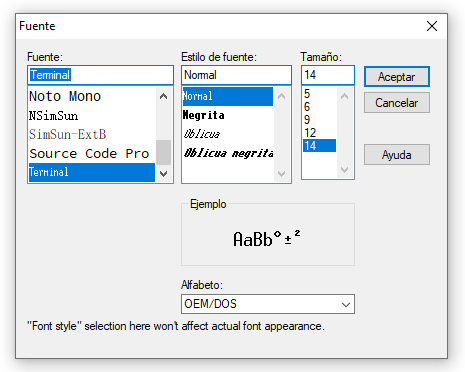
\includegraphics[width=0.6\textwidth]{./imagenes/teraterm_font.png}
  \caption{Tamaño y tipo de letra de la terminal}
  \label{F:teraterm_font}
\end{figure}

La configuración realizada se pierde cada vez que el programa es cerrado, por lo tanto, cada vez que se abre el mismo debería realizarse la misma configuración nuevamente. Para evitar esto es posible guardar la configuración actual, para ello es necesario ir a Setup->Save setup..., una ventana se abrirá y podrá guardarse un archivo llamado \entreComillas{TERATERM.INI}, guardarlo reescribe la configuración anterior, por lo tanto, si no desea perderla, debería guardar el archivo de configuración ya existente antes de sobrescribirlo.

Algunos programas pueden ser cargados desde la terminal. Esto es usado, por ejemplo, para cargar programas escritos en Basic, al intérprete de Basic corriendo en el microprocesador, el cual es discutido en el capítulo~\ref{C:SistemaMedio}: \nameref{C:SistemaMedio}, sección~\ref{C:programas_del_sistema_medio}: \nameref{C:programas_del_sistema_medio}.

Para realizar esta tarea se tiene que ir a File->Send file... y seleccionar el archivo que contiene el programa a ser enviado a través de la terminal (ver figura~\ref{F:teraterm_send_file}). Como el microprocesador requiere de un período de tiempo mínimo para poder procesar un carácter recibido, no es posible enviarlos todos de seguido sin establecer un retardo entre cada uno de ellos; por esta razón Tera Term posee una configuración para esto en Setup->Serial port..., en la ventana de configuración pueden configurarse los retardos entre caracteres y líneas; en la figura~\ref{F:teraterm_transmit_delay} se indica dónde colocar estos valores.

\begin{figure}[H]
\centering
\subfloat[Opción de envío de archivo]{
	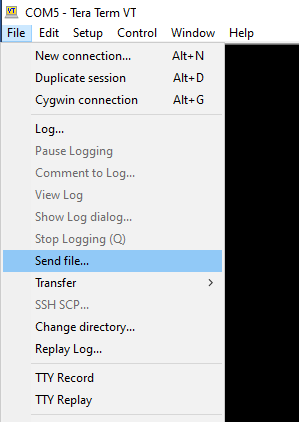
\includegraphics[width=0.35\textwidth]{./imagenes/teraterm_send_file.png}
	\label{F:teraterm_send_file}}
\quad
\subfloat[Configuración de delay]{
	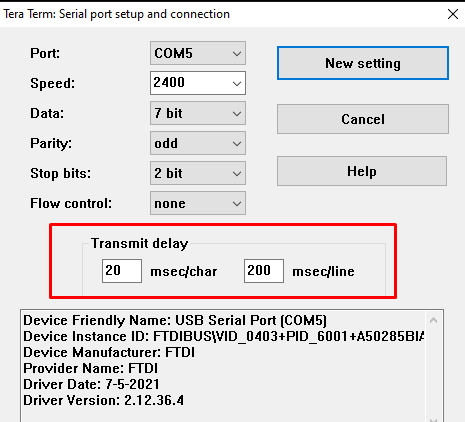
\includegraphics[width=0.45\textwidth]{./imagenes/teraterm_transmit_delay.png}
	\label{F:teraterm_transmit_delay}}
\caption{Cargado de programas a través de la terminal}
\label{F:send_file}
\end{figure}

Para que este proceso funcione correctamente debe respetarse el carácter ASCII utilizado para representar un salto de línea. Dado que distintos formatos de texto utilizan diferentes caracteres para esto (algunos utilizan retorno de carro CR, del inglés \textit{Carriage Return}, o salto de línea LF, del inglés \textit{Line Feed}). Estos no necesariamente son los que el programa ejecutándose en el microprocesador interpreta como salto de línea, a veces es necesario modificarlos. Para ello se utilizó el programa discutido en la siguiente sección, \nameref{C:multicomander}.

\section{Multi Commander}
\label{C:multicomander}

Multi Commander \cite{multicommander} es un programa para el manejo de archivos y se utiliza como alternativa al explorador de Windows. Sin embargo, es de interés para este proyecto únicamente la herramienta para cambiar los caracteres utilizados para representar saltos de línea en archivos de texto. En la figura~\ref{F:multicommander} se puede observar dónde encontrar esta herramienta dentro del programa.

\begin{figure}[H]
  \centering
  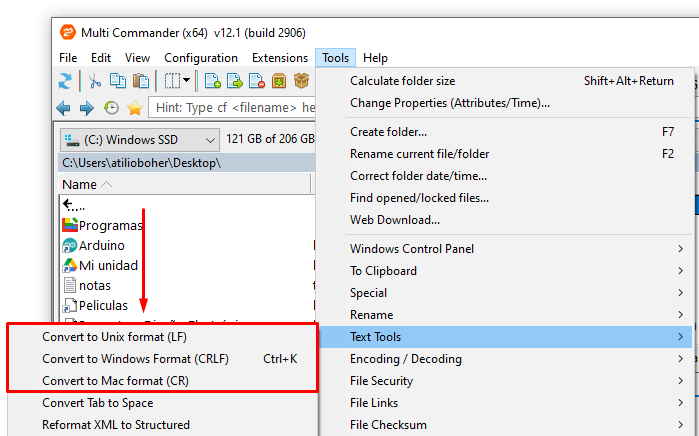
\includegraphics[width=0.85\textwidth]{./imagenes/multicommander.png}
  \caption{Herramienta para cambio de carácter de salto de línea en Multi Commander}
  \label{F:multicommander}
\end{figure}


\section{Programador universal XGecu TL866-3G}
\label{C:Programador}

Para el grabado de la memoria se utilizó el programador universal XGecu TL866-3G (figura~\ref{F:programador_universal}). Para ello fue necesaria la descarga e instalación del software correspondiente al mismo, el cual puede ser encontrado en la página oficial del fabricante \cite{pagina_de_descarga_programador}. Se recomienda descargar la opción 2 \entreComillas{DownLoad From Local Server}.

\begin{figure}[ht!]
  \centering
  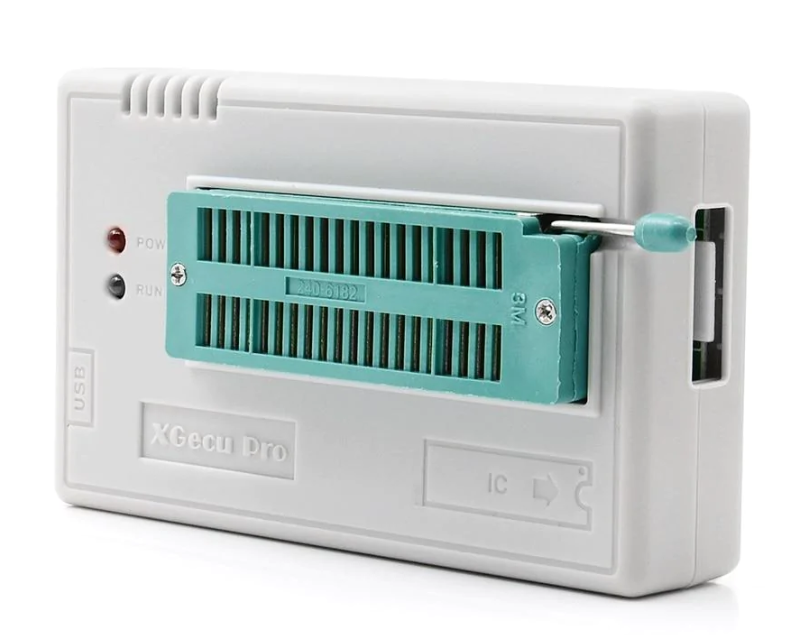
\includegraphics[width=0.6\textwidth]{./imagenes/programador_universal.png}
  \caption{Programador universal XGecu TL866-3G}
  \label{F:programador_universal}
\end{figure}

En la figura~\ref{F:programador_universal_opciones} puede verse el entorno gráfico del programa. Con la flecha~1 se encuentra indicado donde seleccionar la memoria a ser grabada o leída. En este proyecto fueron utilizadas las memorias AT28C64\cite{datasheet_AT28C64} y X28C256\cite{datasheet_X28C256}, ambas disponibles en la librería del programador. Con la flecha~2 se indica una función para el testeo de chips lógicos digitales, herramienta que fue de utilidad en varias ocasiones.

\begin{figure}[ht!]
  \centering
  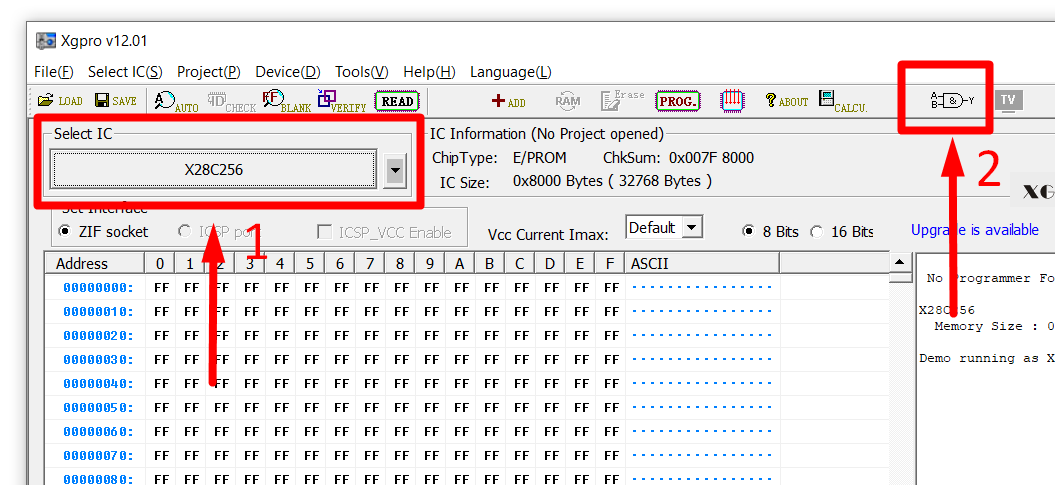
\includegraphics[width=0.85\textwidth]{./imagenes/programador_universal_opciones.png}
  \caption{Entorno gráfico del programa del programador universal XGecu TL866-3G}
  \label{F:programador_universal_opciones}
\end{figure}

\clearpage
\section{KiCad EDA}

Para la construcción de los circuitos electrónicos del presente proyecto se utilizó el software KiCad, un software libre para el diseño electrónico automatizado (del inglés: Electronic Design Automation EDA) de circuitos electrónicos. 
Entre las aplicaciones más destacadas del software se encuentran:  el editor de esquemas, el editor de circuitos impresos y el selector de huellas impresas para los componentes utilizados, entre otras. 
KiCad es un software de código abierto y gratuito, el cual puede ser descargado de su página oficial \cite{kicad_page}. En línea pueden encontrarse video-tutoriales muy completos para el uso adecuado del mismo.
La versatilidad de la herramienta mencionada ha proporcionado simpleza al momento de confeccionar los esquemáticos y los diagramas de circuito impreso para las placas del proyecto. A modo de ejemplo en las figuras~\ref{F:esquema_kikad} y~\ref{F:pcb_kikad} se encuentran el editor de esquemas y el editor de circuitos impresos del software KiCad. 

\begin{figure}[ht!]
  \centering
  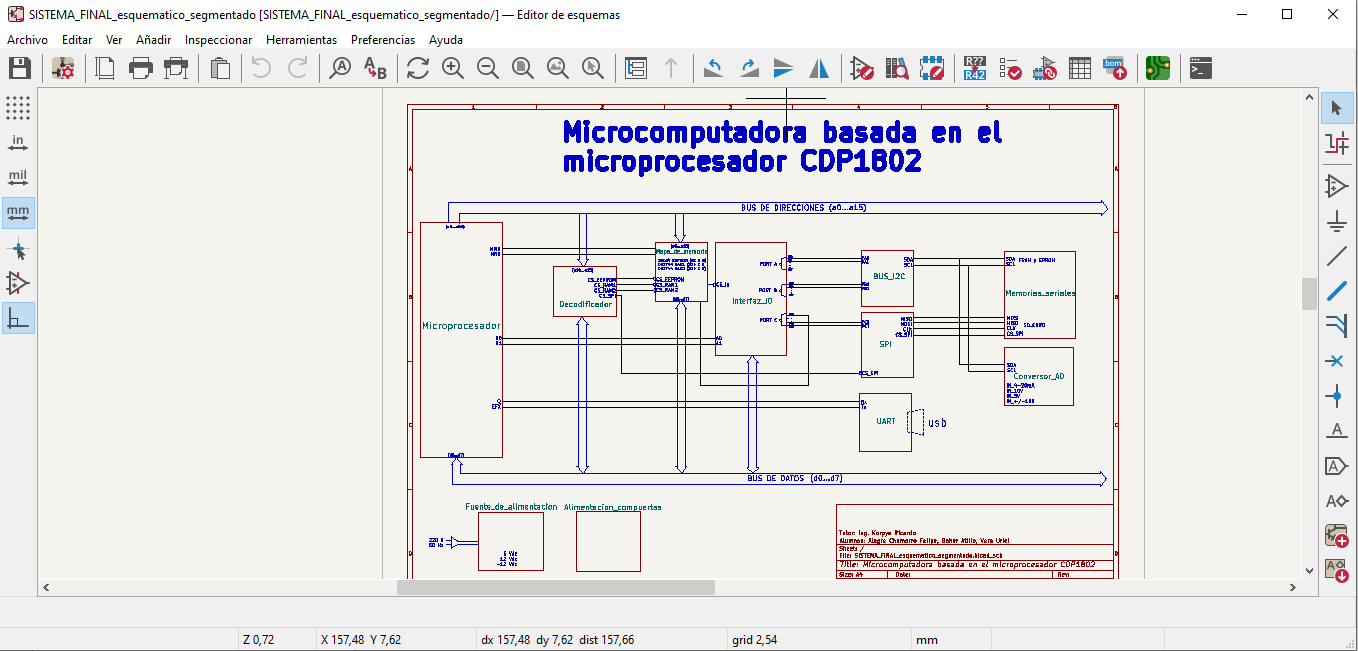
\includegraphics[width=0.95\textwidth]{./imagenes/esquema_kikad.png}
  \caption{Entorno gráfico del editor de esquemas del software KiCad}
  \label{F:esquema_kikad}
\end{figure}

Una herramienta destacada para el diseño de los circuitos impresos es el editor de huellas y de símbolos, lo cual es útil a la hora de confeccionar un esquemático o un PCB cuando se posee un dispositivo cuyo símbolo o huella no está incluida dentro de las librerías del programa. KiCad cuenta con un entorno adecuado para el dibujo y desarrollo de los elementos mencionados, permitiendo agregar a las librerías los mismos. Esta solución realza la aplicabilidad del programa y ha sido de gran utilidad para el desarrollo del trabajo.

\begin{figure}[ht!]
  \centering
  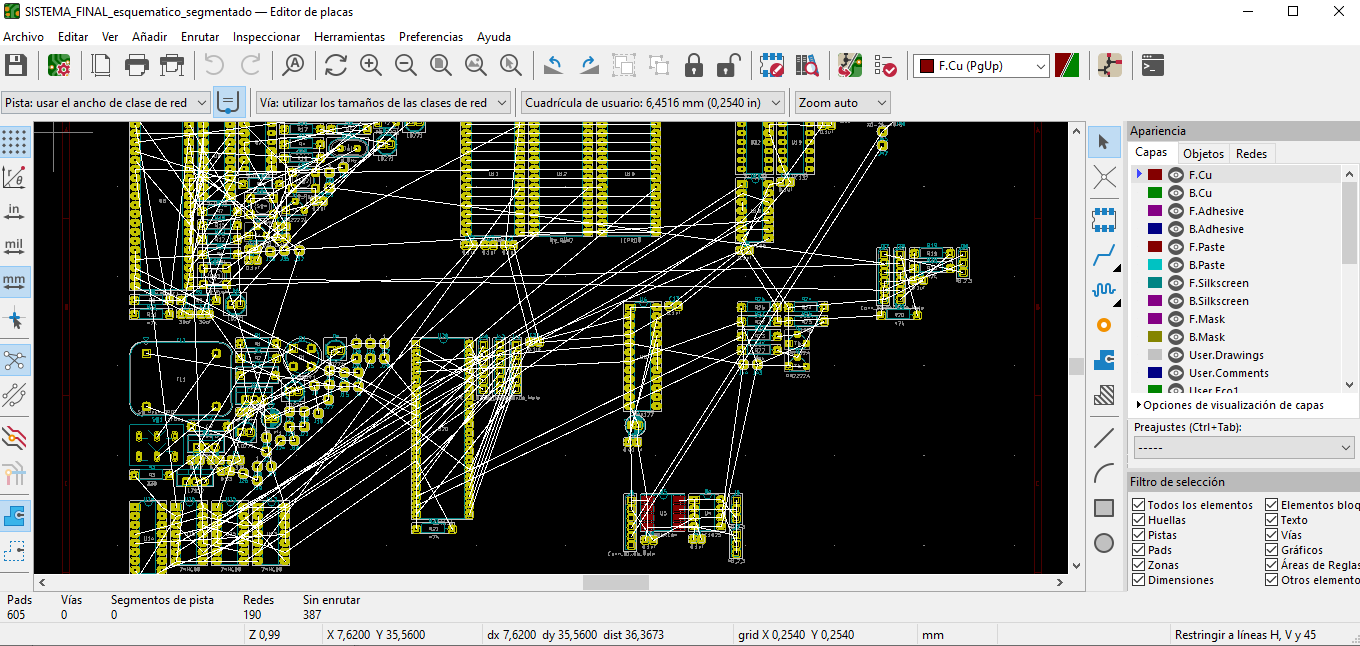
\includegraphics[width=0.95\textwidth]{./imagenes/pcb_kikad.png}
  \caption{Entorno gráfico del editor de circuito impreso del software KiCad}
  \label{F:pcb_kikad}
\end{figure}